% Document settings and packages
\documentclass[a4paper,12pt]{report}
	\usepackage[utf8]{inputenc}
	\usepackage{graphicx}
	\usepackage{hyperref}
	\usepackage{url}
	\usepackage{geometry}
	\usepackage[acronym]{glossaries}
	\graphicspath{{figures/}}
	
% Acronyms page
\makeglossaries
\newacronym{vpn}{VPN}{Virtual Private Network}
\newacronym{ip}{IP}{Internet Protocol}
\newacronym{ipv4}{IPv4}{Internet Protocol version 4}
\newacronym{ipv6}{IPv6}{Internet Protocol version 6}
\newacronym{tcp}{TCP}{Transmission Control Protocol}
\newacronym{udp}{UDP}{User Datagram Protocol}
\newacronym{gre}{GRE}{Generic Routing Encapsulation}
\newacronym{tls}{TLS}{Transport Layer Security}
\newacronym{ipsec}{IPsec}{Internet Protocol Security}
\newacronym{ssh}{SSH}{Secure Shell}
\newacronym{l2tp}{L2TP}{Layer 2 Tunneling Protocol}
\newacronym{osi}{OSI}{Open Systems Interconnection}
\newacronym{dtls}{DTLS}{Datagram Transport Layer Security}
\newacronym{mipv6}{MIPv6}{Mobile IPv6}
\newacronym{ietf}{IETF}{Internet Engineering Task Force}
\newacronym{sa}{SA}{Security Association}
\newacronym{esp}{ESP}{Encapsulating Security Payload}
\newacronym{ah}{AH}{Authentication Header}
\newacronym{spd}{SPD}{Security Policy Database}
\newacronym{sad}{SAD}{Security Association Database}
\newacronym{pad}{PAD}{Peer Authorization Database}
\newacronym{spi}{SPI}{Security Parameter Index}
\newacronym{isakmp}{ISAKMP}{Internet Security Association and Key Management Protocol}
\newacronym{icv}{ICV}{Integrity Check Value}
\newacronym{ike}{IKE}{Internet Key Exchange}
\newacronym{iana}{IANA}{Internet Assigned Numbers Authority}
\newacronym{nat}{NAT}{Network Address Translation}
\newacronym{iv}{IV}{Initialization Vector}



\begin{document}
	\begin{titlepage}
		\newgeometry{top=15mm}
		\begin{center}
			\vspace{-10in}
			{\LARGE University of Bucharest \\
			Faculty of Mathematics and Computer Science }
			\vfill
			\textbf{\huge Virtual Private Networks} \\
			\vspace{5mm}
			{\Large Bogdan Ionescu} \\
			\vspace{20mm}
			\begin{flushleft}{\large Supervisor \\
			Lect. Dr. Eng. Paul Irofti}
			\end{flushleft}
			\vfill
			\today
		\restoregeometry
		\end{center}
	\end{titlepage}
	\author{Bogdan Ionescu}
	\date{\today}
	\tableofcontents
	
	% Print acronyms page
	\setlength{\glsdescwidth}{\hsize}
	\glsaddall
	\printglossary[type=\acronymtype,nonumberlist,style=long]
	
	\chapter{Virtual Private Networks}
	\section{Importance of VPNs}
		
	In this day and age, networking is everywhere, especially considering the exceedingly fast expansion of the Internet. The Internet, the ultimate network of networks, has radically changed our day-to-day life. Just several years ago, simple everyday habits, such as quickly searching for a piece of information on Google, online shopping, streaming your favorite songs or paying your bills with just a few clicks would have seemed possible only in a distant future. And yet here we are today, achieving even more impressive tasks, making use of all kinds of networks available within our laptops, phones, tablets and even home electronics, thanks to the IoT.
		
		Unfortunately, the Internet's rapid development also comes with a few important drawbacks which are regrettably often overlooked --- the most significant one being cybersecurity. \textit{Cybersecurity} is the protection of computer systems and networks from the theft and damage of hardware, software or electronic data, as well as from the disruption of the services they provide. Most often, networks, full of information, are the first frontier when trying to exploit systems,  which is why network security represents such an important key aspect against cybercrime.
		
		Inevitably, when having any communication over the Internet, a significant amount of data is being sent between you (more precisely, your device) and the other party, commonly a server or another person's device. Although this data can sometimes be quite harmless, such as a quick Google search for a cake recipe or just streaming some music, in some cases it may contain more sensitive and valuable information than you can think of. Personal messages while chatting with a close friend, credit card information when making an online payment, passwords used when logging in to different websites, the video feed recorded by your webcam when having an online conference --- these are only just a few examples of what kind of infomation leaves your private home network when accessing the Internet. Since the Internet is a public network, such data can be easily intercepted by other parties before reaching its destination, which often leads to catastrophic consequences.
		
		By now you might think that if you are using an application which encrypts its data, you should be safe on the Internet. Unfortunately, this is often not the case, as there are many places where things can go wrong. For example, in many messaging systems, messages pass through intermediary parties, such as the application's servers, which store them, from where they are retrieved by the recipient. In such scenarios, data is generally encrypted only in transit --- from the sender to the server, and from the server to the destination. Even if the servers encrypt the data at rest (which, surprisingly, does not always happen), they still must have access to the cryptographic keys used in this process, therefore information is still being vulnerable in case the actual servers are being targeted. Moreover, this allows the third party, or any other organization which has a backdoor to these servers, to freely recognize our data. Such invasion of privacy is prevented by using end-to-end encryption, a system where only the communicating users can read the messages, denying any other third party to access the cryptographic keys needed to decrypt the information.
		
		Even if such encryption is used, with strong cryptographic ciphers, unlikely to be broken in attacks, we still might experience some troubles. Application data that leaves our home network, in order to be routed over networks, will have an \acrfull{ip} header added to it, which contains our public IP address and the destination IP address. These are unique, ISP-issued addresses which can be used to monitor and censor traffic, since every service we try to access will be identified by its IP address. This could also lead to IP address-based geo-blocking and IP range ban, methods often employed by media companies, governments, intelligence agencies and many others.
		
		So far we have only talked about the consequences from the point of view of a casual user, but damages rise significantly in the case of cyber attacks against major businesses, usually leading to huge amounts of loss in revenue. In fact, Juniper Research estimated that the average cost of a data breach in 2020 will exceed \$150 million, as more business infrastructure gets connected \cite{junipercybercrime}. In order to mitigate cyber attacks, they usually maintain one or more private networks inside their offices and only from within these controlled networks employees can access necessary resources. Such resources can actually be part of the same network, thus making transfer of data safe, since everything happens inside the private network, but inevitably some resources, such as cloud services, will be accessed through the Internet. Some employees must also be able to connect to the private network through the Internet even if they are part of another network, in order to access its resources, possibly in case of time-critical emergencies or just to work remotely from their homes. Therefore, many companies need a technology that allows secure communication between their private network and another host across a public network, or even to another different private network, such as communication between two private networks owned by different offices of the same company, located in distant regions.
		
		The solution to all the aforementioned problems, and to many other vulnerabilities while using a public network, is a \acrfull{vpn}.
		
		\section{What Is a Virtual Private Network?}
		Security over networks is usually described by three components: confidentiality, integrity and authenticity. Confidentiality, often achieved by encryption, guarantees that data can only be understood by authorized entities. Integrity ensures that the data has not been modified between these endpoints. Finally, authenticity proves that data originated from an authorized party, and not from another source. Apart from these three, another concept which is often massively desired over public networks refers to anonimity, which assures that information we send out does not divulge our identity. All of these can be achieved by VPNs, if implemented correctly.
		
		A \acrfull{vpn} extends a private network by allowing hosts which are not part of it to send and receive data over a public network, usually the Internet, as if they are directly connected to the private network. VPNs are build by establishing a virtual link of communication between two nodes, one being part of the private network. The second node will forward its traffic to it, the first node acting like a proxy, therefore appearing as the traffic actually originated from within the private network from which it is part of. Since encryption is a common, yet not an inherent part of a VPN connection, this channel of communication is usually called a \textit{tunnel} --- only the two endpoints being able to understand the data passing through it. 
		
		Classified by the type of topology of connections, defined by the location of the two endpoints, VPNs usually are of three types: site-to-site, point-to-point (sometimes also called host-to-host), which are the most common, and a combination of the two, point-to-site.
		
		Site-to-site VPNs, illustrated in figure \ref{fig:site-to-site_VPN}, establish a tunnel between two whole networks, therefore allowing any authorized host in any of the two networks to make use of it. Such architecture is frequently used by businesses to securely connect networks owned by the same company in different regions.
		\begin{figure}[h]
			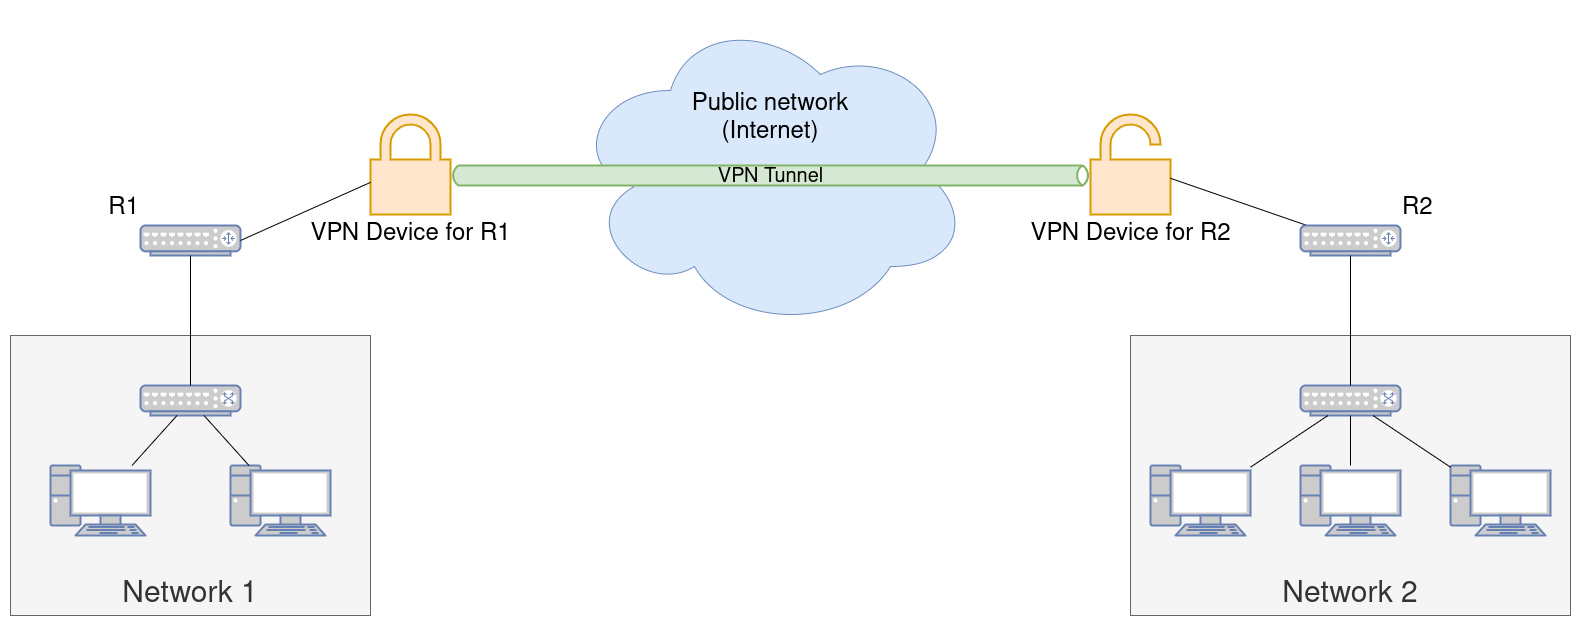
\includegraphics[width=\textwidth]{site-to-site_VPN}
			\centering
			\caption{In this site-to-site architecture, the two VPN devices establish a secure tunnel through the public network. Since traffic must be encrypted from one site to another, the two VPN endpoints, placed in this case after the routers, are responsible for securing data before it crosses the public network. VPN technology can also be directly embedded in routers, removing the need for two additional devices.}
			\label{fig:site-to-site_VPN}
		\end{figure}
		
		Advantages of site-to-site VPNs include scalability, being quite straightforward to add another site, or more devices inside one of the networks, and high availability, as the VPN tunnel does not depend on a device inside the network to initiate and maintain the secure connection. However, for regular users who wish to remain as private as possible, site-to-site VPNs have a quite serious disadvantage. Since traffic is secured just as it leaves the site, by the VPN device or router, data is still vulnerable in the network until it reaches this point, or after it was decrypted, at the other site. As a result, anyone who can intercept our traffic at these stages is a potential threat. Although this scenario is not likely to happen in a business office, it is very probable, for example, for someone who wishes to secure his data from a public place which offers free Internet connection, such as a coffee shop or restaurant.
		
		Point-to-point VPNs (figure \ref{fig:point-to-point_VPN}) establish a secure tunnel between two single hosts in usually separate networks, encryption and decryption taking place only at these points, therefore providing end-to-end encryption and eliminating the aforementioned risk present with site-to-site architectures.
		\begin{figure}[h]
			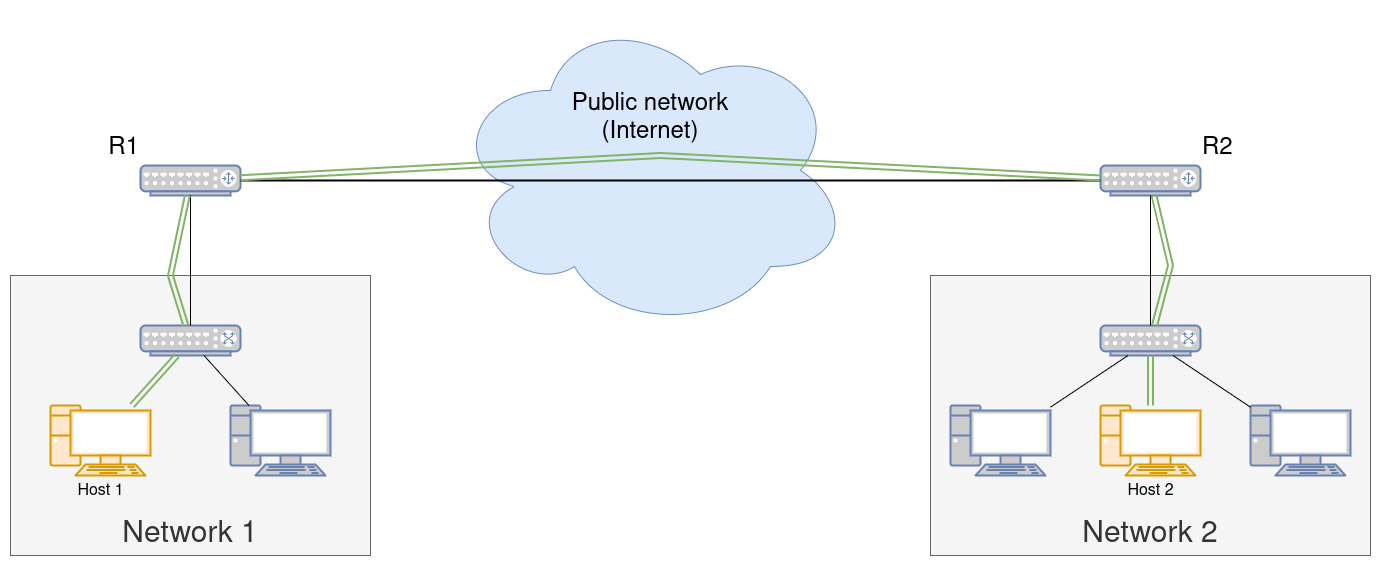
\includegraphics[width=\textwidth]{point-to-point_VPN}
			\centering
			\caption{A point-to-point VPN tunnel between two hosts. The tunnel is usually initiated by one endpoint, but it is dependent on both; if one of the endpoints is down or unreachable, no tunnel can be established.}
			\label{fig:point-to-point_VPN}
		\end{figure}
		
		Point-to-point VPNs are used to form traditional consumer VPNs, where a user establishes a secure tunnel between his device and a server, which is then used as a proxy to access resources, possibly again through the Internet. If this traffic is intercepted, its origin could only be traced back to the proxy server, not the authentic source, which is the other endpoint of the tunnel. This can only be identified by those who have access to the proxy server, in addition to all the decrypted traffic routed through it. Although some VPN service providers claim that they do not log such traffic when clients use their servers, this sometimes is hard to believe. Such risks, along with the fact that VPN providers charge for their services, prompt users to rely on self-hosted VPNs, in which they own the proxy server. In this case, it is the user's job to install and manage the VPN software on both the proxy server and the other endpoint.
		
		\section{Tunneling Protocols}
		The two endpoints of a VPN tunnel do most of the work, being responsible with managing the tunnel and making sure that communication through it is possible. In order for it to actually function, they must modify the regular network packets received from the clients, making sure they are routed to the other endpoint, not to their actual destination, and also provide encryption, if desired. From an original network packet only important information is kept, usually either the network or the transport layer, discarding other layers. This fragment is often called the payload packet, because it is then used as a payload for the final packet. If encryption is used, some portion or the entire payload packet can be modified. This process of encapsulating a packet inside another packet is called \textit{tunneling}, achieved by \textit{tunneling protocols}.
		
		For example, IP in IP \cite{rfc2003} is a tunneling protocol which encapsulates an IP datagram within another IP datagram, as shown in figure \ref{fig:ip-in-ip_packet}. The source IP in the outer IP header will correspond to the entry point of the tunnel, while the destination IP will reveal the exit point, therefore guaranteeing that the packet will be routed to the other VPN endpoint. Except to the encapsulator decrementing the TTL field in the inner IP header, the packet payload remains unchanged during its delivery to the tunnel exit point. Once there, decapsulation takes place, removing the outer IP header and reconstructing the original packet, which will be sent to its original destination.
		\begin{figure}[h]
			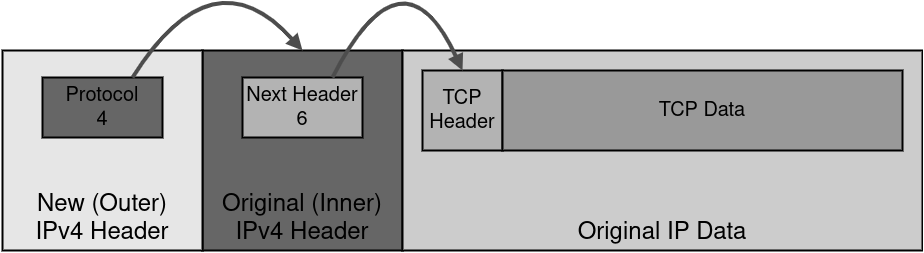
\includegraphics[width=\textwidth]{ip_in_ip}
			\centering
			\caption{IP in IP encapsulates the IP layer (IP header and payload) from the original packet within another IP packet. To differentiate between the two IP headers, the first one is often called the outer IP header.}
			\label{fig:ip-in-ip_packet}
		\end{figure}
		
		\acrfull{gre} \cite{rfc2784}, a protocol fairly similar to IP in IP, developed by Cisco Systems, and Layer 2 Tunneling Protocol (L2TP) \cite{rfc2661} are just another two examples of tunneling protocols frequently used. However, just like IP in IP, all of these protocols do not provide any confidentiality or integrity. They just encapsulate the data received, without modifying it in order to provide encryption. To achieve this, they generally rely on other protocols.
		
		Internet Protocol Security (IPsec) \cite{rfc6071}, Transport Layer Security (TLS) \cite{rfc8446} and Secure Shell (SSH) \cite{rfc4253} are the most often used protocols for secure network services over an insecure network. A key difference between these three protocols is the OSI layer at which they operate. While IPsec is generally considered a network layer protocol, TLS and SSH depend on a reliable stream of bytes and are therefore implemented over TCP, making them layer 5 or above, or just application layer protocols in the TCP/IP suite. The fact that IPsec performs at a lower layer than the rest and it is not dependent on TCP increases its flexibility and capabilities, being able to secure any transport layer protocol, such as UDP. Datagram Transport Layer Security (DTLS) \cite{rfc6347} was also developed to implement TLS over UDP. Tunneling over UDP is sometimes preferred to avoid the TCP meltdown problem (also known as TCP over TCP), in which tunneling a TCP-encapsulating payload induces a dramatic loss in transmission performance (even up to 20\%)\cite{tcpmeltdown}. OpenSSH, an open source suite of secure networking utilities based on SSH avoids the meltdown by decapsulating and re-encapsulating TCP, only sending the payload through the tunnel \cite{opensshmeltdown}.
		
		IPsec, TLS and SSH use a wide variety of strong cryptographic algorithms, providing robust authentication, confidentiality and integrity, amongst many other services. All three of them support tunneling and are currently used to establish and maintain secure tunnels across many networks worldwide. However, the more complex IPsec is still the most viable and preferred option for tunneling, especially for site-to-site VPNs, while TLS and SSH are better for secure remote access, being more straightforward and easier to set up.
		
	\chapter{Internet Protocol Security}
	\section{Description }
		The goal of Internet Protocol Security (IPsec) is to provide security at the network layer, being used worldwide to deploy a variety of VPNs, therefore guaranteeing either secure traffic between networks or in case of remote access, or end-to-end security. It is also often used by other protocols (e.g. L2TP, MIPv6, GRE) to protect some or all of their traffic.
		
		IPsec is not a single protocol, but rather a set of network protocols, each one with critical and specific tasks, working together to achieve the main goal. The complex IPsec protocol suite can be broken into three essential parts which will be thoroughly explained in the next sections:
		\begin{itemize}
			\item \textbf{Security Associations} define the security services and attributes of a connection shared by two network entities
			\item \textbf{Authentication Header} provides connectionless data integrity and data origin authentication for IP datagrams (hereafter referred to as just integrity) \cite{rfc4302}
			\item \textbf{Encapsulating Security Payload} can provide both data confidentiality and integrity, and limited traffic flow confidentiality \cite{rfc2406}
		\end{itemize}
		
		IPsec has two main modes of operation which define how AH and ESP behave, namely transport mode and tunnel mode. When transport mode is used, only the IP payload is encapsulated and secured by one or both security headers. Tunnel mode encapsulates the entire IP packet to provide a secure hop between two gateways, quite similar with IP in IP. The latter is used to form traditional VPNs.
		
		Although a decent part of the IPsec stack is already directly embedded into the Linux kernel, guaranteeing efficient packet processing with minimum overhead, some daemons are still required in user space, generally those regarding Security Associations.
		
	\section{Security Associations}
	IPsec provides data confidentiality and integrity through the two fundamental security protocols previously mentioned, the Authentication Header (AH) and Encapsulating Security Protocol (ESP). However, since a VPN device might handle many secure streams of data with different hosts at the same time, when an IP datagram employing AH and/or ESP arrives, how does it know which set of security parameters (cryptographic algorithm, keys, policies etc.) to use for that particular connection? Moreover, both AH and ESP support a wide variety of cryptographic ciphers, and therefore the two endpoints must agree beforehand on which exact algorithm to employ, and perhaps generate and exchange cryptographic keys. As you can see, many more security attributes and policies must be negotiated and bound to a specific connection between entities before establishing and actually using an IPsec tunnel. This is the purpose of Security Associations. 
	
	A Security Association (SA) is a relationship between two or more network entities that describe how the entities will utilize security services to communicate securely. This relationship is represented by a set of information that can be considered a contract between the entities, agreed upon and shared between them \cite{rfc2408}. 
	
	An SA describes only one-way traffic, so, in order to secure typical bi-directional communication between two IPsec-enabled systems, a pair of SAs (one in each direction) is required \cite{rfc4301}. Information is stored in a database, where each SA is uniquely identified by a triple consisting of a Security Parameter Index (SPI), an IP Destination Address, and a security protocol (AH or ESP) identifier. The SPI is a random generated 32-bit value used by a receiver to identify the SA to which the incoming packet should be bound (the IP address and protocol will be automatically inferred from the packet headers), and is a mandatory field in the ESP and AH headers.
	
	A model defined in RFC 4301 outlines three databases in order to store various SA information: the Security Policy Database (SPD), the Security Association Database (SAD), and the Peer Authorization Database (PAD) \cite{rfc4301}.
	
	\subsection{Security Policy Database}
		A Security Policy Database (SPD) specifies processing rules for different IP datagrams received by the device. The SPD is consulted during processing of all inbound or outbound traffic, including traffic not protected by IPsec, that traverses the IPsec boundary. For a given packet, three processing rules are defined and stored in the database:
		\begin{itemize}
			\item DISCARD: Packets that match this rule will be immediately discarded by the device.
			\item BYPASS: Packets that match this rule are allowed to cross the IPsec boundary, not needing any further IPsec processing.
			\item PROTECT: Packets that match this rule are afforded IPsec protection. In this case, the SPD usually points to an SAD entry which defines the security services to be employed (AH and/or ESP), as well as their attributes (e.g. mode of operation, algorithm).
		\end{itemize}
		
	\subsection{Security Association Database}
		To determine what to do with a particular datagram, a device first checks the SPD, in order to see if the datagram should be discarded, allowed to pass through unchanged or offered security services. If the latter is the case, the SAD is interrogated to find the particular security mechanisms to be applied.
		
		More formally, a Security Association Database stores the parameters associated
with one particular SA. For outbound processing, each SAD entry is pointed to by entries in the SPD cache.  For inbound processing, for unicast SAs, the SPI is used either alone to look up an SA or in conjunction with the IPsec protocol type \cite{rfc4301}.

	RFC 4301 describes which data items must be in an SAD entry:
	\begin{itemize}
		\item Security Parameter Index (SPI).
		\item Sequence Number Counter: a 64-bit counter used to generate the Sequence Number field in AH or ESP headers.
		\item Sequence Counter Overflow: flag indicating whether overflow of the sequence number counter should prevent transmission of additional packets on the SA, or whether rollover is permitted.
		\item Anti-Replay Window: a 64-bit counter used to determine whether an inbound AH or ESP packet is a replay
		\item AH Authentication algorithm, key, etc.
		\item ESP encryption algorithm, key, mode, IV, etc.
		\item ESP integrity algorithm, keys, etc.
		\item ESP combined mode algorithms, key(s), etc.
		\item Lifetime of the SA: a time interval after which an SA must be replaced with a new SA (and new SPI) or terminated.
	\end{itemize}
	
	\subsection{Peer Authorization Database}
	The Peer Authorization Database (PAD) simply provides a link between the SPD and a security association management protocol, such as IKE or KINK, along with other constraints and information related to their peers.
	
	
	\subsection{Internet Key Exchange}
		Internet Key Exchange (IKE) is one of the most often used protocols used to establish, negotiate, modify and delete Security Associations between IPsec nodes. Unlike AH and ESP, IKE is not directly embedded into the Linux kernel, and therefore a daemon in user space is required. Such applications generally implement IKE version 2 (IKEv2), an improvement over the initial IKE version 1 (IKEv1). A draft for IKE version 3 (IKEv3) exists, but it is not yet adopted.
		
		IKE is partly based on three other designs:
		\begin{itemize}
			\item Internet Security Association and Key Management Protocol (ISAKMP), a framework defining procedures and packet formats to establish, negotiate, modify and delete SAs
			\item OAKLEY Key Determination Protocol, a generic key exchange protocol
			\item SKEME, a versatile key exchange technique which provides anonymity, repudiability, and quick key refreshment
		\end{itemize}
		
		Since both AH and ESP almost always require an SA, IKE is the first protocol employed, representing an initial step towards a secure connection. In order to actually establish an IPsec SA, IKE goes through two phases. 
		
		IKE phase 1 is used as a setup stage where the peers agree on how to exchange further information securely. This is done through an ISAKMP SA negotiation, which establishes a secure channel of communication, much needed by phase 2. During this ISAKMP session, the IPsec nodes are authenticated, through either a pre-shared key, digital signature, or public key encryption \cite{rfc5996}, an encryption algorithm and hash algorithm are chosen, and a Diffie-Hellman group is created.
		
		In IKE phase 2 the secure tunnel previously established is used to safely negotiate the actual IPsec SA, where the parameters for AH and ESP are decided. 
		
		IKE is usually implemented over UDP on port 500.
		
		\section{Authentication Header}
		\subsection{Description}
		Authentication Header (AH) is one of the two core protocols of the IPsec suite. Its main objective is to provide integrity for IP datagrams, term which is used to embody two critical concepts:
		\begin{itemize}
			\item \textbf{Connectionless integrity} guarantees that the essential information contained within a packet has not been changed in transit, either by a malicious entity or due to errors
			\item \textbf{Data origin authentication} ensures the IP datagram originated from a trusted source
		\end{itemize}
		
		This is achieved by employing a cryptographic hash algorithm, used to compute an integrity check value (ICV) over the majority of the IP datagram. The calculated ICV is then added in an AH header which is inserted in the outgoing packet. The receiving IPsec device repeats the ICV computation, and compares it with the one in the AH header. If the two values differ, the packet was modified in transit and is discarded.
		
		\subsection{Format}
		The AH format (figure \ref{ah_header}) is quite simple, containing the following fields:
	\begin{itemize}
	\item Next Header (8 bits) is used to link headers together and identifies the next protocol used after AH. The value is chosen from the set of IP Protocol Numbers defined by IANA. For example, a value of 4 indicates IPv4, a value of 41 indicates IPv6, and a value of 6 indicates TCP.
	\item Payload Length (8 bits) specifies the length of AH in 32-bit words (4-byte units), minus 2. Therefore, for example,  if an integrity algorithm yields a 96-bit authentication value, this length field will be the value 4 (3 32-bit word fixed fields plus 3 32-bit words for the ICV, minus 2) \cite{rfc4302}.
	\item Reserved (16 bits) is not currently used and it is set to zero. 
	\item Security Parameter Index (32 bits) identifies the SA to which an incoming packet is bound.
	\item Sequence Number (32 bits) is a counter field that is initialized to zero when an SA is formed between two devices, and then incremented for each datagram sent using that particular SA. This uniquely identifies each datagram on an SA and is used to provide protection against replay attacks by preventing the retransmission of captured datagrams \cite{kozierok2005tcp}.
	\item Authentication Data (variable size in order to support different hashing algorithms, but it must be a multiple of 32 bits) contains the ICV. The entire header must be a multiple of either 32 bits (for IPv4) or 64 bits (for IPv6), so additional padding may be added to the Authentication Data field if necessary.
\end{itemize}			
		
		\begin{figure}[h]
			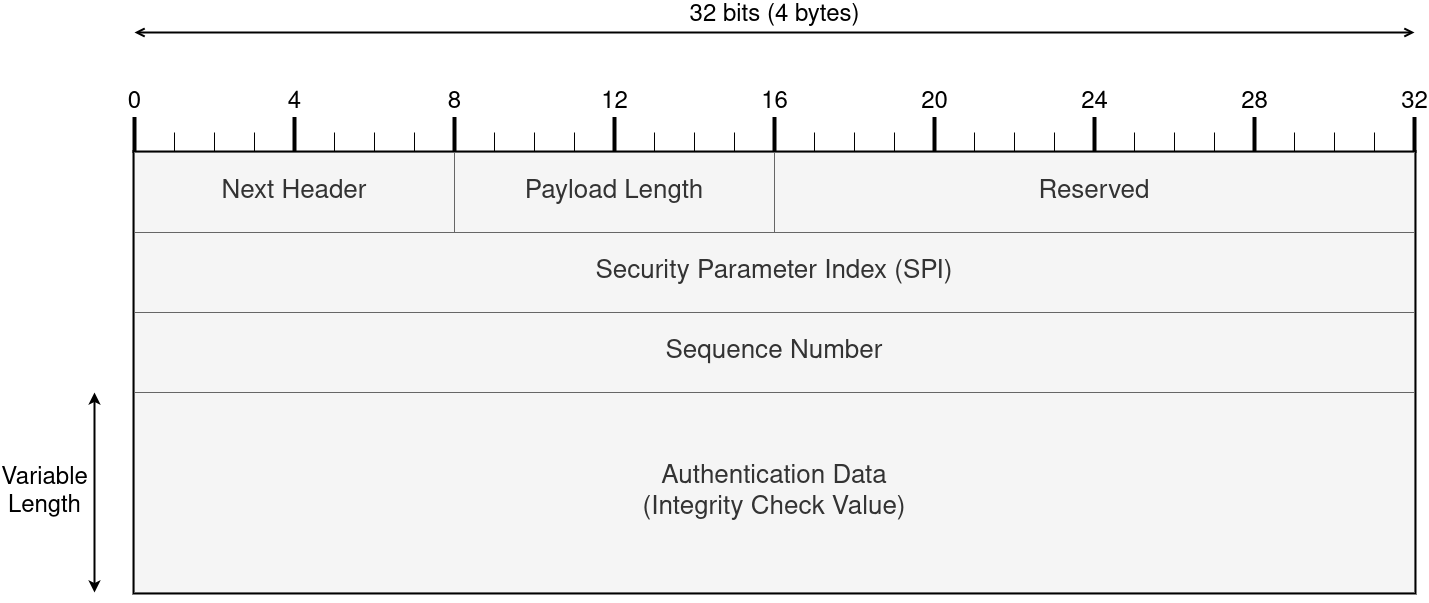
\includegraphics[width=\textwidth]{ah_header}
			\centering
			\caption{IPsec Authentication Header (AH) format}
			\label{ah_header}
		\end{figure}
		
		\subsection{Placement}
		AH placement depends on the IPsec mode of operation and the IP version used (IPv4 or IPv6).
		\subsubsection{Transport Mode}
		\begin{figure}[h]
			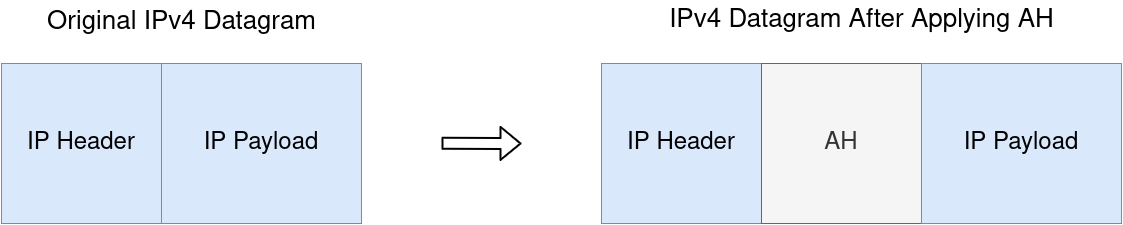
\includegraphics[width=\textwidth]{ah_transport_ipv4}
			\centering
			\caption{In the context of IPv4, AH is placed after the IP header (and any options that it contains), but before the next layer protocol \cite{rfc4302}.}
		\end{figure}
		
		\begin{figure}[h]
			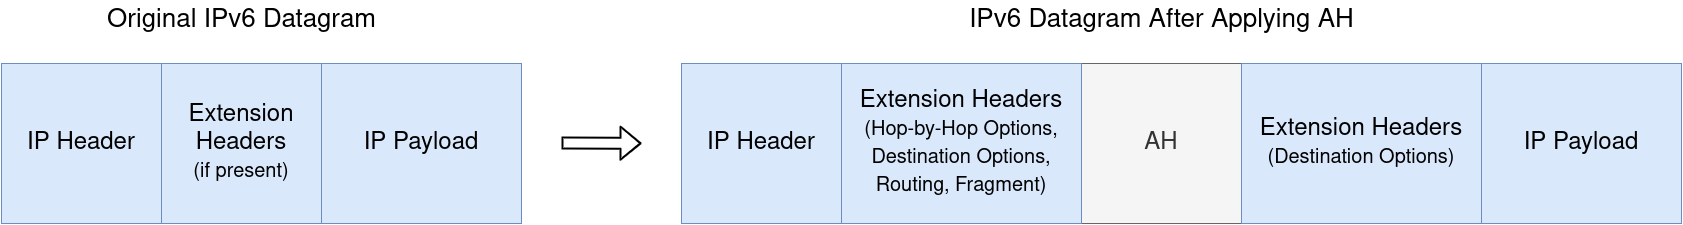
\includegraphics[width=\textwidth]{ah_transport_ipv6}
			\centering
			\caption{In the IPv6 context, AH is viewed as an end-to-end payload, and thus should appear after hop-by-hop, routing, and fragmentation extension headers.  The destination options extension header(s) could appear before or after or both before and after the AH header depending on the semantics desired \cite{rfc4302}.}
		\end{figure}
		
		\subsubsection{Tunnel Mode}
		As previously mentioned, when employing IPsec in tunnel mode, the whole IP datagram (not just the payload) is encapsulated within another IP datagram. The inner IP header carriers the final IP source and destination addresses, while the outer IP header contains the addresses of the IPsec gateways. The latter can also contain special routing options that dictate how the packet will traverse the public network. Mixed inner and outer IP versions are allowed, i.e., IPv6 over IPv4 and IPv4 over IPv6 \cite{rfc4302}.
		\begin{figure}[h]
			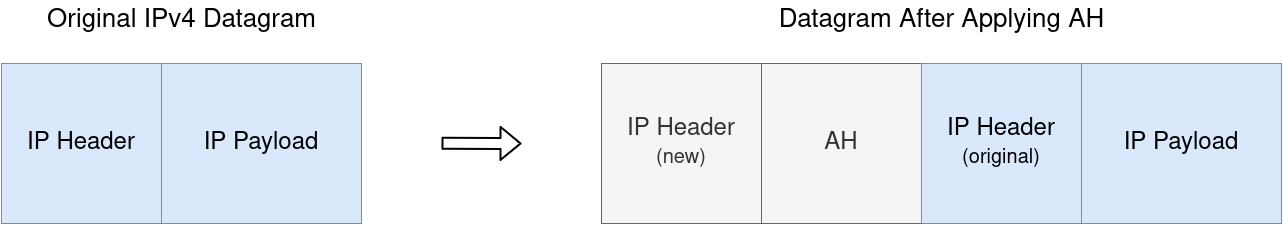
\includegraphics[width=\textwidth]{ah_tunnel_ipv4}
			\centering
			\caption{AH with IPv4.}
		\end{figure}
		
		\begin{figure}[h]
			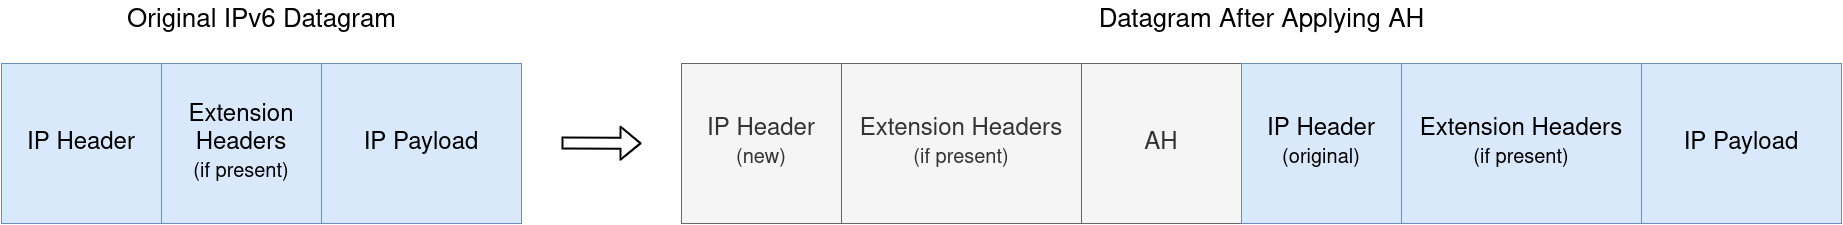
\includegraphics[width=\textwidth]{ah_tunnel_ipv6}
			\centering
			\caption{AH with IPv6.}
		\end{figure}
		
		\subsection{ICV Computation}
		The ICV is calculated over the majority, but not the entire IP datagram. Fields which are modified in transit between the two gateways must be excluded in order for the receiving IPsec peer to not mistakenly discard the packet (remember that even if a single bit is changed the ICV values will differ). An example is the time to live (TTL) field in the IPv4 header, which is decremented at each hop until the datagram reaches its destination, or until it reaches zero, in which case the datagram is discarded. With this in mind, the AH ICV is computed over the following:
		\begin{itemize}
			\item Everything after the AH header.
			\item The AH header (the ICV is initially set to zero).
			\item IP or extension headers fields before the AH header that are immutable in transit. For example, in IPv4, the DSCP, ECN, flags, fragment offset, TTL and header checksum fields are excluded.
		\end{itemize}
	
		\subsection{NAT Incompatibility}
			A considerable disadvantage of AH is that it is incompatible with Network Address Translation (NAT). As previously explained, the AH header incorporates the IP source and destination addresses in the ICV computation. If one of the IPsec gateways is inside a private network, as is usually the case, the ICV will be calculated over a private IP address. Just as the packet leaves into the public network, Network Address Translation (NAT) will inevitably modify the IP header in order for it to contain only public addresses, therefore invalidating the ICV. Although some methods to bypass NAT in case of AH packets exist \cite{rfc3715}, they are quite limited. Fortunately, integrity can also be provided by ESP. IPsec ESP tunnels do not cover the outer IP header within the message integrity check, and so will not cause problems with address translation.
			
		\section{Encapsulating Security Protocol}
		\subsection{Description}
		IPsec AH provides integrity services to IP datagrams, guaranteeing that the packets received by the IPsec peers are intact and not maliciously altered in transit. However, for most applications, this is only one small piece of the puzzle. Although potential eavesdroppers would not be able to change the intercepted IP datagrams, they still can examine their contents. This includes the authentic IP addresses of the communicating peers (present in the only IP header in transport mode, and in the inner IP header in tunnel mode), as well as the transport data, which probably contains the most valuable information in a network packet, such as HTTP data. Therefore, for perfect privacy, AH is clearly not enough. This is where IPsec ESP steps in.
		
		Encapsulating Security Payload (ESP) is the second core protocol of the IPsec suite, and probably the most versatile, implementing a mix of security services in IPv4 and IPv6. ESP can be used to provide confidentiality, data origin authentication, connectionless integrity, an anti-replay service, and (limited) traffic flow confidentiality \cite{rfc4303}.
		
		ESP can be used in conjunction with AH, the first one providing confidentiality while the latter guarantees integrity. However, since ESP can implement both services (i.e. the packets will be protected with regard to confidentiality and integrity), AH is deemed unnecessary in most situations.
		
		\subsection{Format}
		ESP provides confidentiality to IP datagrams by encrypting them. To achieve this, ESP repackages the original IP datagrams using a special format. Instead of having just a header and a payload, ESP fields are divided into four components:
		\begin{itemize}
			\item \textbf{ESP Header.} This contains the SPI and Sequence Number fields, and comes before the encrypted data.
			\item \textbf{ESP Payload Data.} The encrypted payload data encapsulated by ESP. Depending on the mode of operation, this could either be an upper layer message or an IP datagram. If the encryption scheme employed requires an Initialization Vector (IV), this is added at the beginning.
			\item \textbf{ESP Trailer.} This section is placed after the encrypted data. It contains padding and two fields, Pad Length and Next Header. Padding is required in order to support encryption algorithms that require the data to be encrypted to have a certain block size. It is also used to make sure the ESP layer is a multiple of 32 bits. The Pad Length field indicates the padding size, in order for the receiver to clearly separate the original message from the padding. Next Header contains the protocol number of the next header in the encapsulated payload.
			\item \textbf{ESP Authentication Data.} This is optional and is only present if integrity services are also employed by ESP for that particular SA. It contains the ICV calculated over the ESP header, payload and trailer. Unlike AH, this does not include the outer IP header in tunnel mode.
		\end{itemize}
		
		\begin{figure}[h]
			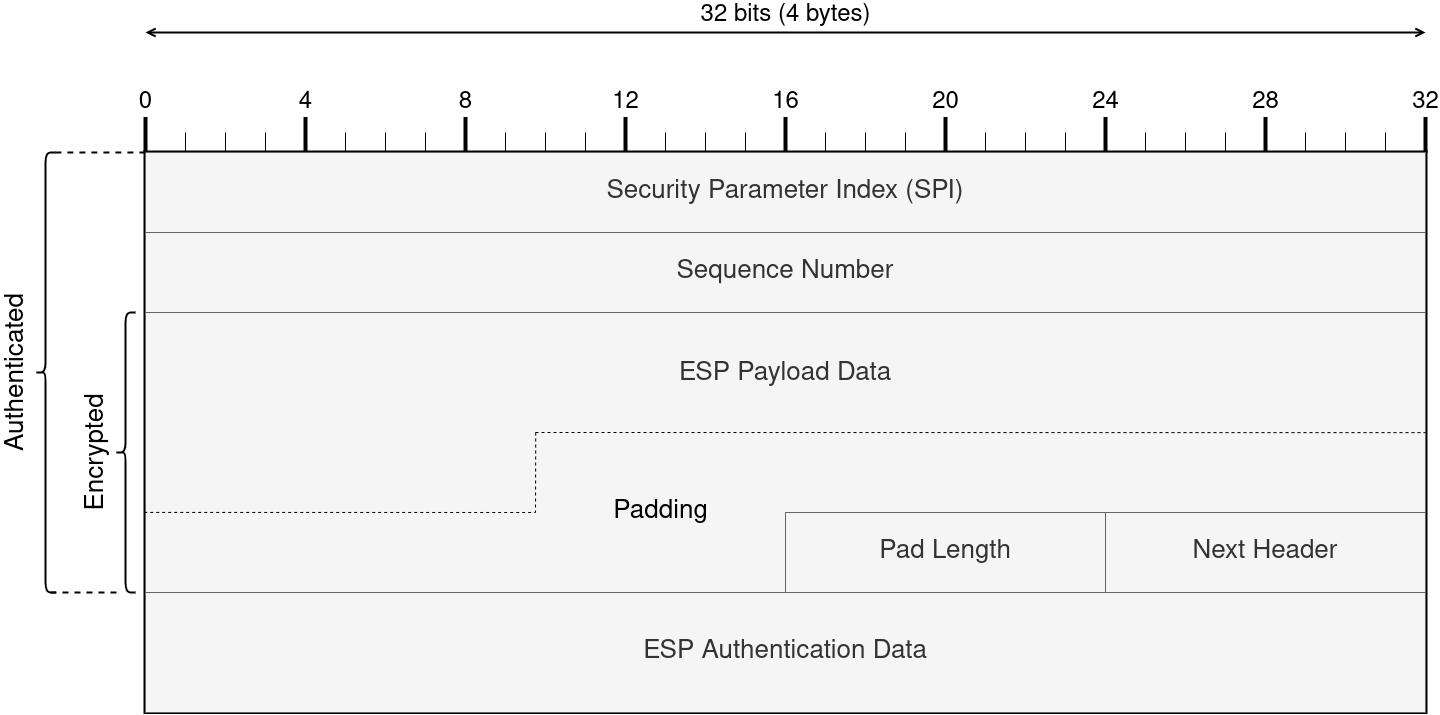
\includegraphics[width=\textwidth]{esp_format}
			\centering
			\caption{ESP Fields Format.}
		\end{figure}
\newpage
		\subsection{Placement}
		\subsubsection{IPv4}
		
		\begin{figure}[!htb]
			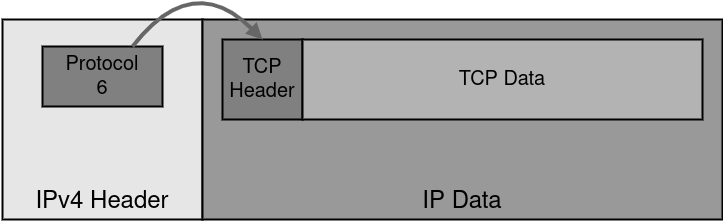
\includegraphics[width=\textwidth,height=0.15\textheight,keepaspectratio]{original_ipv4_packet}
			\centering
			\caption{Original IPv4 datagram with TCP as the upper layer protocol.}
		\end{figure}
		
		\begin{figure}[!htb]
			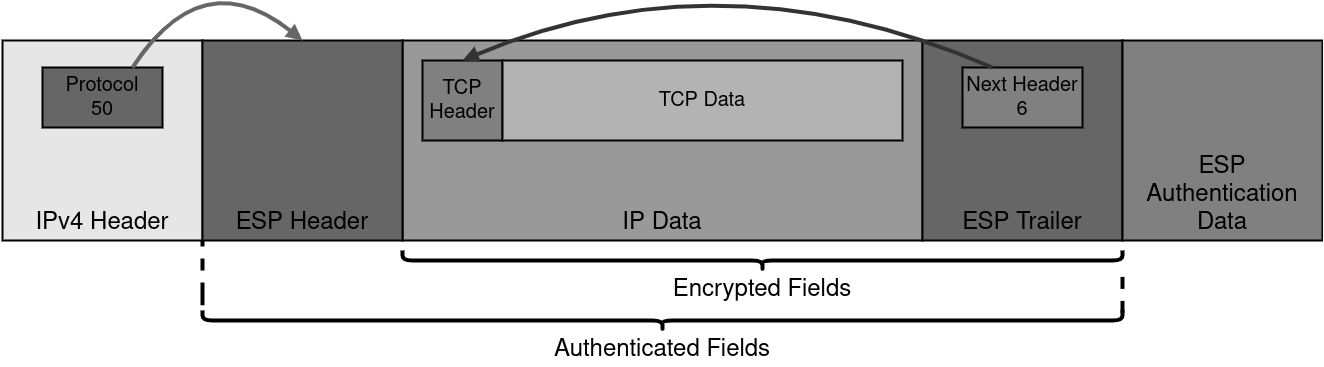
\includegraphics[width=\textwidth]{esp_ipv4_transport}
			\centering
			\caption{In transport mode, the ESP header is inserted after the IPv4 header and before the next layer protocol, protecting the upper layer message.}
		\end{figure}
		
		\begin{figure}[!htb]
			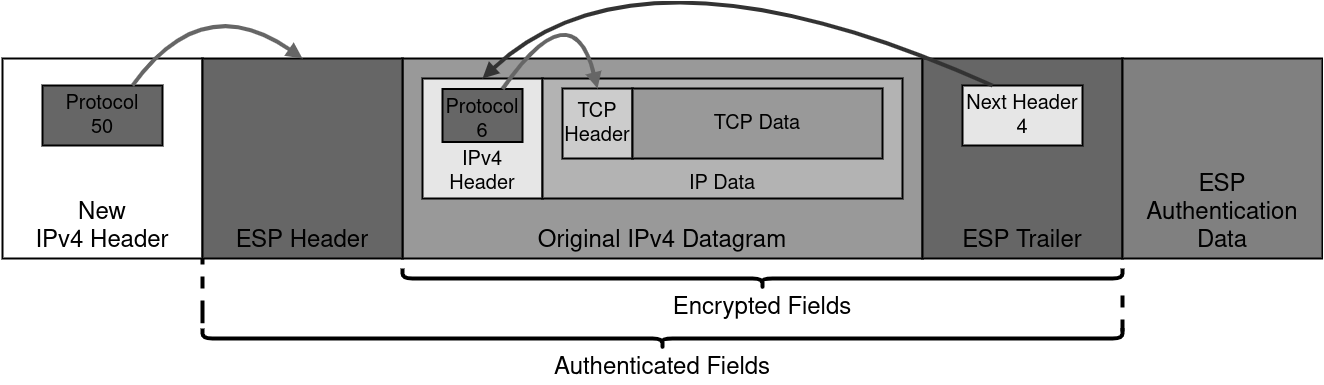
\includegraphics[width=\textwidth]{esp_ipv4_tunnel}
			\centering
			\caption{In tunnel mode, ESP encapsulates and protects the entire original IPv4 datagram.}
		\end{figure}
\newpage
		\subsubsection{IPv6}
		\begin{figure}[!htb]
			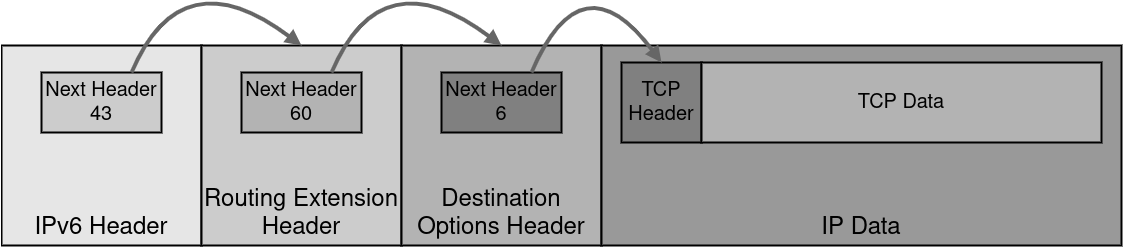
\includegraphics[width=\textwidth,height=0.15\textheight,keepaspectratio]{original_ipv6_packet}
			\centering
			\caption{Original IPv6 datagram, including Routing Extension Header and Destination Options Extension Header, with TCP as the upper layer protocol.}
		\end{figure}
		
		\begin{figure}[!htb]
			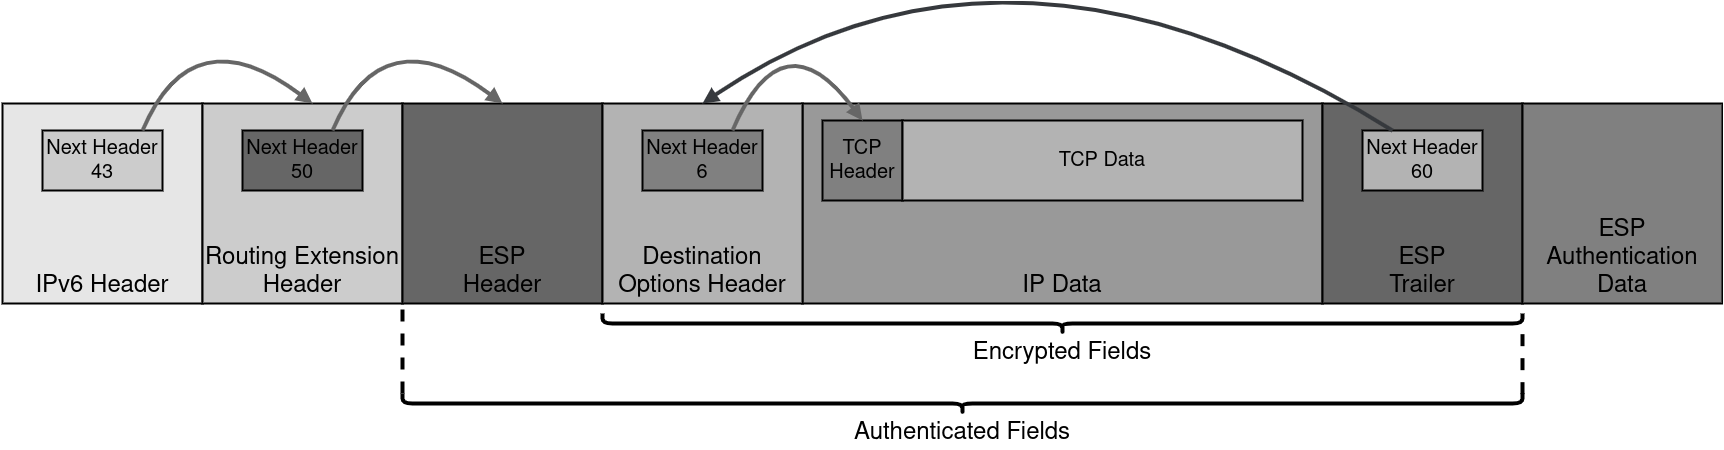
\includegraphics[width=\textwidth]{esp_ipv6_transport}
			\centering
			\caption{In transport mode, ESP should appear after hop-by-hop, routing, and fragmentation extension headers.  Destination options extension header(s) could appear before, after, or both before and after the ESP header depending on the semantics desired \cite{rfc4303}.}
		\end{figure}
		
		\begin{figure}[!htb]
			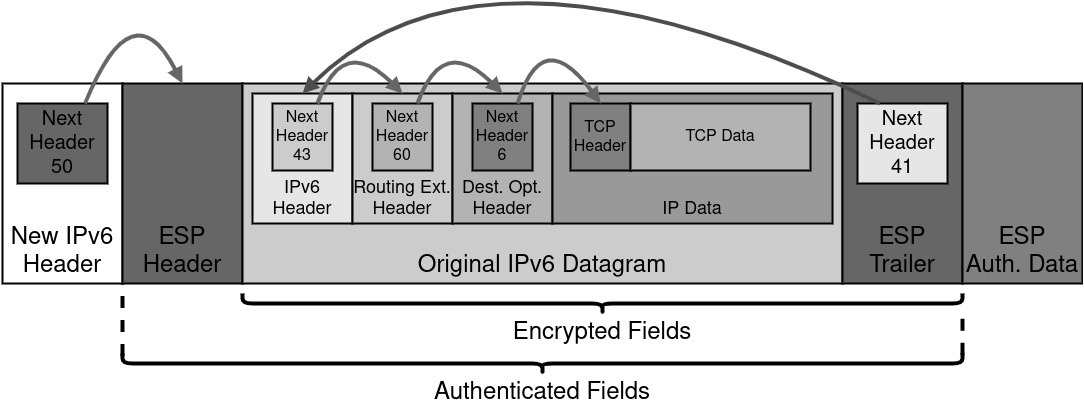
\includegraphics[width=\textwidth]{esp_ipv6_tunnel}
			\centering
			\caption{In tunnel mode, ESP protects the entire original IPv6 datagram.}
		\end{figure}
		
% Print bibliography
\bibliographystyle{abbrv}
\bibliography{bibliography}


\end{document}